\subsection{其他的结构}
前一节讲了最简单的聚合物结构-线性均聚物。对于各种各样的体系结构包括那些具有实际和学术意义的体系都可以得到类似的结果。在本节中,我们导出了在空间变化势作用下分支均聚物(branched homopolymers)、嵌段共聚物和接枝共聚物(block and graft copolymers)的显式表达式。像聚合物的结构是化学无序的,如随机分支均聚物(randomly branched homoploymers)、统计共聚物(statistical copolymers)和随机接枝共聚物(randomly grafted copolymers)的讨论,将推迟到$4.7$节讨论。
\subsubsection{分支均聚物}
作为分支均聚物的第一个例子,我们考虑一个$3$臂星形均聚物,如图\ref{三臂星形均聚物}所示。每个臂采用连续高斯链模型描述并且有任意的长度。相应的,每条链的聚合度分别是$N_1$,$N_2$,$N_3$。假设每个臂上的片段经历一个化学势场$w (\mathbf{r})$。在这种情况下,因为每个臂在化学上是相同的,所以只需要一种化学势。
\begin{figure}[H]
\centering
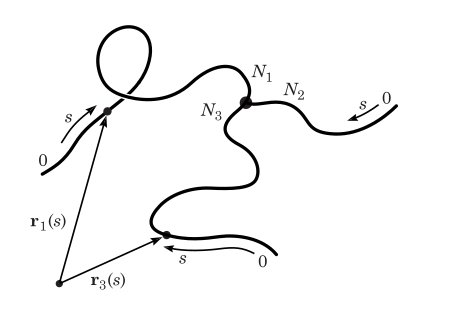
\includegraphics[scale=0.7]{./figures/34.png}
\caption{连续高斯链模型中的$3$臂星形聚合物。聚合度分别为$N_1$,$N_2$,$N_3$的三个支臂连接在一个中心支点上。第$j$个臂的构型用空间曲线$\mathbf{r}_j(s)$描述,$s\in [0,N_j]$。}
\label{三臂星形均聚物}
\end{figure}

如图\ref{三臂星形均聚物}所示,第$j$个臂$(j=1,2,3)$的构型由空间曲线$\mathbf{r}_j(s)$描述,其中路径参数$0\leq s\leq N_j$,这是从每个臂的自由端测量。在支点处,臂满足$\mathbf{r}_1(N_1)=\mathbf{r}_2(N_2)=\mathbf{r}_3(N_3)$。

第$3.1.2$节关于线性均聚物的公式可以很容易地推广到目前的情况。微观段密度(microscopic segment density)可以写成
\begin{equation}
\tilde{\rho}(\mathbf{r})=\sum_{j=1}^3 \int_{0}^{N_j}\, \mathrm{d}s\rho(\mathbf{r}-\mathbf{r}_{j}(s))
\end{equation}
与施加的化学势$w (\mathbf{r})$的相关的势能是整个聚合物形状$\mathbf{r}$的一个泛函,$\mathbf{r}(s)\equiv \left\{ \mathbf{r}_1(s),\mathbf{r}_2(s),\mathbf{r}_3(s) \right\}:$
\begin{equation}
\beta U_1[\mathbf{r},w]=\int \mathrm{d}\mathbf{r}^{'}w(\mathbf{r}^{'})\tilde{\rho}(\mathbf{r}^{'})
\end{equation}
归一化的配分函数$Q[w]$也可以表示为路径积分的比率
\begin{equation}
Q[w]\equiv \frac{Z[w]}{Z_0}=\frac{\int^{*}\mathcal{D}\mathbf{r}\exp (-\beta U_0[\mathbf{r}]-\beta U_1[\mathbf{r},w])}{\int^{*}\mathcal{D}\mathbf{r}\exp (-\beta U_0[\mathbf{r}])} \label{82}
\end{equation}
其中理想链的势能
\begin{equation}
\beta U_0[\mathbf{r}]=\frac{3}{2b^2}\sum_{j=1}^3\int_{0}^{N_j} \mathrm{d}s\left| \frac{d\mathbf{r}_j(s)}{ds} \right|^2
\end{equation}
和$\int^{*}\mathcal{D}\mathbf{r}$是受支点约束的三个臂上的路径积分
\begin{equation}
\int^{*}\mathcal{D}\mathbf{r}\equiv \int \mathcal{D}\mathbf{r}\delta (\mathbf{r}_1(N_1)-\mathbf{r}_2(N_2))\delta (\mathbf{r}_2(N_2)-\mathbf{r}_3(N_3))  \label{83}
\end{equation}
方程(\ref{82})中的路径积分可以通过离散这三条路径来计算,这三条路径对应于星臂的构型,从而得到了一个类似于线性均聚物方程$(3.21)$的表达式。方程(\ref{83})的约束是通过建立从三个臂的自由端开始,在公共分支点的位置终止的路径积分,因此,由乘积$q(\mathbf{r},N_1)q(\mathbf{r},N_2)q(\mathbf{r},N_3)$给出了有支点的星形聚合物关于$\mathbf{r}$的统计重量,其中传播子(propagators)满足方程$(3.25)-(3.26)$。配分函数是
\begin{equation}
Q[w]=\frac{1}{V}\int \mathrm{d}\mathbf{r}~q(\mathbf{r},N_1;[w])q(\mathbf{r},N_2;[w])q(\mathbf{r},N_3;[w])
\end{equation}
应该注意,应用这个公式并不需要解出扩散方程$(3.25)$的三个独立解,而是一个,因为对$0\leq s\leq N_{\max}$(其中$N_{\max}$是$N_j$中最大的)的$q(\mathbf{r},s;[w])$足以评估全部的三个传播子。

$3$臂星形均聚物的段密度算子可与线性聚合物的方程$(3.55)$类比得出。在连续高斯链模型中,我们有
\begin{equation}
\rho(\mathbf{r};[w])=-\frac{1}{Q[w]}\frac{\delta Q[w]}{\delta w(\mathbf{r})}=\rho _1(\mathbf{r};[w])+\rho _2(\mathbf{r};[w])+\rho _3(\mathbf{r};[w])
\end{equation}
这里的$\rho _j(\mathbf{r};[w])$表示星的第$j$个臂对平均段密度的贡献。其中
\begin{equation}
\rho _{j}(\mathbf{r};[w])=\frac{1}{VQ[w]} \int_{0}^{N_j}\, \mathrm{d}s\,q_{j}(\mathbf{r},N_{j}-s;[w])q(\mathbf{r},s;[w]) \label{87}
\end{equation}
“互补传播子”$q_{j}(\mathbf{r},s;[w])$满足与$q$相同的扩散方程,但具有不同的初始条件,即
\begin{equation}
\frac{\partial}{\partial s}q_j(\mathbf{r},s;[w])=\frac{b^2}{6}q_j(\mathbf{r},s;[w])-w(\mathbf{r})q_j(\mathbf{r},s;[w]) \label{88}
\end{equation}
\begin{equation}
q_j(\mathbf{r},0;[w])=
\begin{cases}
q(\mathbf{r},N_2;[w])q(\mathbf{r},N_3;[w]), & j=1 \\
q(\mathbf{r},N_1;[w])q(\mathbf{r},N_3;[w]), & j=2 \\
q(\mathbf{r},N_1;[w])q(\mathbf{r},N_2;[w]), & j=3  \label{89}
\end{cases}
\end{equation}

\begin{figure}[H]
\centering
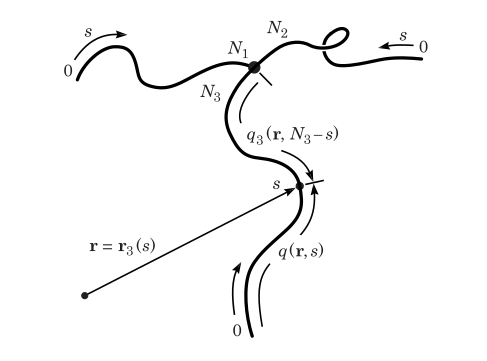
\includegraphics[scale=0.7]{./figures/35.png}
\caption{$3$臂星形均聚物的密度算子$\rho _3(\mathbf{r};[w])$的构造。这个密度由统计权重$q(\mathbf{r},s;[w])$组成,代表臂$3$的自由端,具有互补的传播子$q_3(\mathbf{r},N_3-s;[w])$,表示臂与分支点连接的部分的统计重量。在满足初始条件(\ref{89}),后者是通过对远离分支点的方程(\ref{88})进行积分获得的。}
\label{三臂星形图像}
\end{figure}

图(\ref{三臂星形图像})说明了当$j=3$时的臂的平均密度$\rho _3$的方程(\ref{87})的物理解释。臂必须通过点$\mathbf{r}=\mathbf{r}_3(s)$,其中$s$是从臂的自由端测量的路径参数。与这种臂构型相关联的是统计重量$q(\mathbf{r},s;[w])$的乘积,它表示臂的悬空(自由)末端,以及权重$q_{3}(\mathbf{r},N_{3}-s;[w])$,表示与星其余部分相连的臂段。互补传播子$q_3$是从分支点开始,在$N_3-s$的总的路径距离上对方程(\ref{88})积分得出的。这种积分的初始条件是在分支点与剩余的两个臂相关联的统计权重,它可以用两个$q$传播子的乘积表示,如方程(\ref{89})所述。

上述结果可以很容易地推广到具有任意臂数的星形均聚物。最一般情况是具有不同长度且$p\geq3$臂的星形均聚物,总段密度算子的求值要求扩散方程的$p+1$个解:一种是从长度为$N_{\max}$(最长臂长)的链获得$q$,另一解为$p$互补传播子$q_j(\mathbf{r},s;[w])$,$s\in [0,N_j]$。在具有等臂长的$p$星聚合物的特殊情况下,由于所有互补传播子相同,计算量大大减少。因此,在这种高对称性的特殊情况下,只需要扩散方程的两个解。

\begin{figure}[H]
\centering
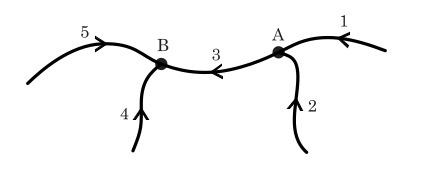
\includegraphics[scale=0.7]{./figures/36.png}
\caption{另一个例子,一个分支均聚物由$5$部分组成,$1-5$连接在两个分支点$A$和$B$上。箭头表示一个(任意)的积分方向,以建立聚合物的统计重量。}
\label{AB嵌段}
\end{figure}

作为分支均聚物的第二个例子,我们考虑了图(\ref{AB嵌段})所示的支化聚合物。聚合物由标记为$1-5$的五个节段组成,分别连接在$A$和$B$的两个支点处。第$j$节的聚合度用$N_j$表示。没有什么特殊的方法来建立这样一种聚合物的统计重量,但各种替代品提供了同等的结果。为了说明如何通过在分支点$B$处合成传播子来计算归一化配分函数$Q[w]$,图(\ref{AB嵌段})中聚合物截面上的箭头指示了用于计算传播子的积分方向,箭头是任意分配的。有图明显看出,在$B$处,三个方向都聚焦在此,通过将第$3$,$4$和$5$段中的传播子组合在一起可以得到$Q[w]$
\begin{equation}
Q[w]=\frac{1}{V}\int \mathrm{d}\mathbf{r}q_3(\mathbf{r},N_3;[w])q(\mathbf{r},N_4;[w])q(\mathbf{r},N_5;[w])
\end{equation}
第$4$段和第$5$段中,$q$传播子在自由链端开始,因此满足方程$(3.25)-(3.26)$。相反,第3节的$q_3$传播子在分支点$A$处开始,从而满足初始条件下的扩散方程(\ref{88})
\begin{equation}
q_3(\mathbf{r},0;[w])=q(\mathbf{r},N_1;[w])q(\mathbf{r},N_2;[w])
\end{equation}
这个初始条件提供了与支点$A$处的链节$1$和$2$相关联的统计权重。

类似的表达式可以写成对这种支化聚合物的平均段密度的各种贡献。例如,第$3$段对段密度运算符的贡献可以表示为
\begin{equation}
\rho(\mathbf{r};[w])=\frac{1}{VQ[w]}\int _{0}^{N_3} \mathrm{d}sq_{3c}(\mathbf{r},N_3-s;[w])q_3(\mathbf{r},s;[w])
\end{equation}
其中$q_3(\mathbf{r},s;[w])$是从分支点$A$出发的传播子。“互补”传播子$q_{3c}(\mathbf{r},N_3-s;[w])$在分支点$B$处发起,并扩展路径距离$N_3-s$在$\mathbf{r}$点加入传播子$q_{3c}$。在初始条件下,$q_{3c}$满足方程(\label{传播子求导})
\begin{equation}
q_{3c}(\mathbf{r},0;[w])=q(\mathbf{r},N_4;[w])q(\mathbf{r},N_5;[w])
\end{equation}
它提供了分支点$B$处的分支$4$和$5$的统计权重。

利用相关的参数,可以构造具有外势的任意结构的分支均聚物的配分函数以及密度算子和应力算子。这种表达式也可以推广到连续高斯链之外,在离散和蠕虫状链模型的背景下处理分支聚合物。

\subsubsection{嵌段接枝共聚物}
嵌段共聚物和接枝共聚物是聚合物工业中特别重要的材料,与纳米技术特别相关。由于这种聚合物是由两个或两种以上的在化学性质上不同的部分(“blocks”或“grafts”)组成的,它们在势场存在的情况下的统计力学比均聚物更丰富。

我们首先讨论$AB$两嵌段共聚物的连续高斯链模型,如图$\ref{图37}$所示。共聚物的总聚合物度指数为$N$,$0\leq s \leq fN$(实线)段由$A$型段组成,$fN \leq s \leq N$(虚线)由B型段组成。$f$是表示$A$链长度与总链长度之比的参数,如果进一步定义$A$和$B$段具有相等的体积,则$f$对应于链上$A$型段的平均体积分数。与共聚物的$A$和$B$段相对应的统计段长度分别是$b_A$和$b_B$。我们还引入了外部化学势场$w_A(\mathbf{r})$和$w_B(\mathbf{r})$,它们分别作用于共聚物的$A$和$B$段。

\begin{figure}[H]
\centering
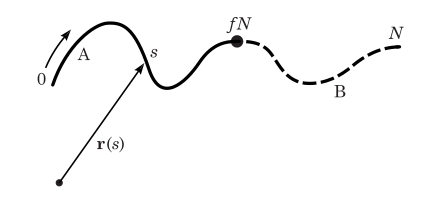
\includegraphics[scale=0.7]{./figures/37.png}
\caption{$AB$两嵌段共聚物的连续高斯链模型。$0\leq s \leq fN$(实线)段由$A$型段组成,$fN \leq s \leq N$(虚线)由$B$型段组成。$f$是表示$A$链长度与总链长度之比的参数。}
\label{图37}
\end{figure}

这种两嵌段共聚物的拉伸势能可以表示为
\begin{equation}
\beta U_0[\mathbf{r}]=\int_{0}^{N} \mathrm{d}s\frac{3}{2[b(s)]^2}\left| \frac{d\mathbf{r}(s)}{ds} \right|^2
\end{equation}
这里
\begin{equation}
b(s)\equiv
\begin{cases}
b_A, & 0\leq s \leq fN \\
b_B, & fN \leq s \leq N\\
\end{cases}
\end{equation}
同样,与外部势$w_A$和$w_B$相关的势能可以写为
\begin{equation}
\beta U_1[\mathbf{r},w_A,w_B]=\int \mathrm{d}\mathbf{r}^{'}[w_A(\mathbf{r}^{'})\tilde{\rho}_{A}(\mathbf{r}^{'})+w_B(\mathbf{r}^{'})\tilde{\rho}_{B}(\mathbf{r}^{'})]
\end{equation}
其中$\tilde{\rho} _A$和$\tilde{\rho} _B$是由下面公式定义的微观段密度
\begin{equation}
\tilde{\rho} _A(\mathbf{r})=\int _0^{fN} \mathrm{d}s~\delta(\mathbf{r}-\mathbf{r}(s)),~~~\tilde{\rho} _B(\mathbf{r})=\int _{fN}^{N} \mathrm{d}s~\delta(\mathbf{r}-\mathbf{r}(s))
\end{equation}
此两嵌段的归一化配分函数表达式是
\begin{equation}
Q[w_A,w_B]\equiv\frac{Z[w_A,w_B]}{Z_0}=\frac{\int \mathcal{D}\mathbf{r}~\exp(-\beta U_0[\mathbf{r}]-\beta U_1[\mathbf{r},w_A,w_B])}{\int \mathcal{D}\mathbf{r}~\exp(-\beta U_0[\mathbf{r}])}
\end{equation}
前几节所描述的方法也可于将分配函数、密度和应力算子与满足Fokker-Planck方程的链传播算子联系起来。在这种情况下,由共聚物的$s=0$(A节点)端引发的传播子$q(\mathbf{r},s;[w_A,w_B])$满足扩散方程
\begin{equation}
\frac{\partial}{\partial s}q(\mathbf{r},s;[w_A,w_B])=\frac{[b(s)]^2}{6}\triangledown ^2q(\mathbf{r},s;[w_A,w_B])-w(\mathbf{r},s)q(\mathbf{r},s;[w_A,w_B]) \label{3.99}
\end{equation}
这里
\begin{equation}
w(\mathbf{r},s)\equiv
\begin{cases}
w_A(\mathbf{r}), & 0\leq s \leq fN \\
w_B(\mathbf{r}), & fN \leq s \leq N\\
\end{cases}
\end{equation}
方程(\ref{3.99})在初始条件$q(\mathbf{r},0;[w_A,w_B])=1$的情况下求解。

另一个有用的量是从共聚物的$s=N$末端出发的互补传播子$q_c(\mathbf{r},s;[w_A,w_B])$。通过建立从$B$端开始的共聚物统计重量,可以得$q_c$满足类似的扩散方程
\begin{equation}
\frac{\partial}{\partial s}q_c(\mathbf{r},s;[w_A,w_B])=\frac{[b_c(s)]^2}{6}\triangledown ^2q_c(\mathbf{r},s;[w_A,w_B])-w_c(\mathbf{r},s)q_c(\mathbf{r},s;[w_A,w_B]) \label{101}
\end{equation}
这里
\begin{equation}
b_c (s)\equiv
\begin{cases}
b_B, & 0\leq s \leq (1-f)N \\
b_A, & (1-f)N \leq s \leq N\\
\end{cases}
\end{equation}
和
\begin{equation}
w_c (\mathbf{r},s)\equiv
\begin{cases}
w_B(\mathbf{r}), & 0\leq s \leq (1-f)N \\
w_A(\mathbf{r}), & (1-f)N \leq s \leq N\\
\end{cases}
\end{equation}
用$q_c(\mathbf{r},0;[w_A,w_B])=1$,方程(\ref{101})在$s$中也是向前积分的。		

使用上面的传播子,可以用两种等效的方法计算配分函数:
\begin{equation}
\begin{aligned}
Q[w_A,w_B] & = \frac{1}{V}\int \mathrm{d}~\mathbf{r}q(\mathbf{r},N;[w_A,w_B]) \\
&=\frac{1}{V}\int \mathrm{d}~\mathbf{r}q_c(\mathbf{r},N;[w_A,w_B]) \\
\end{aligned}	
\end{equation}
换句话说,两嵌段共聚物的传播子可以从分子的$A$端或$B$端建立,从而得到整个链的等效统计重量。因此,只需求解方程(\ref{3.99})或方程(\ref{101})就能计算配分函数$Q[w_A,w_B]$。

相反,计算两嵌段共聚物的密度算子需要两个链传播子的信息。$A$段和$B$段的平均密度是由现在熟悉的前向和后向传播子组成的过程构造的,从而得到表达式
\begin{equation}
\begin{aligned}
\rho _A(\mathbf{r};[w_A,w_B]) & =-\frac{1}{Q[w_A,w_B]}	\frac{\delta Q[w_A,w_B]}{\delta w_A(\mathbf{r})} \\
& =\frac{1}{VQ[w_A,w_B]} \int _{0}^{fN}\,\mathrm{d}s~q_c(\mathbf{r},N-s;[w_A,w_B])q(\mathbf{r},s;[w_A,w_B]) \\
\end{aligned}	
\end{equation}

\begin{equation}
\begin{aligned}
\rho _B(\mathbf{r};[w_A,w_B]) & =-\frac{1}{Q[w_A,w_B]}	\frac{\delta Q[w_A,w_B]}{\delta w_B(\mathbf{r})} \\
& =\frac{1}{VQ[w_A,w_B]} \int _{fN}^{N}\,\mathrm{d}s~q_c(\mathbf{r},N-s;[w_A,w_B])q(\mathbf{r},s;[w_A,w_B]) \\
\end{aligned}	
\end{equation}
上述结果在嵌段共聚物理论中都是众所周知的(Helfand and Wasserman,1976;Hong and Noolandi,1981;Matsen和Schick,1994a)。

作为最后一个例子,我们讨论$A_2B$接枝共聚物的情况,其结构如图(\ref{3.8})所示。这样的分子可以被看作是有一个$A$主链与一个单一的B块“嫁接”到它。或者,该共聚物可以被看作是一种星共聚物有两个$A$臂,分别是$A_1$和$A_2$,和一个$B$臂。从后一种观点出发,分别用$N_{A1}$,$N_{A2}$和$N_B$来表示臂的聚合程度。为了简单起见,采用了连续高斯链模型。

\begin{figure}[H]
\centering
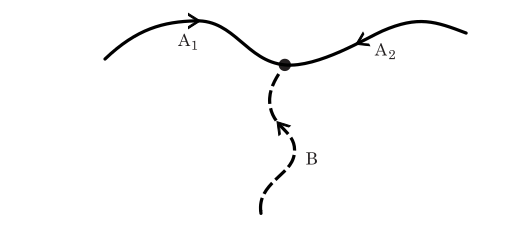
\includegraphics[scale=0.7]{./figures/38.png}
\caption{一个$A_2B$接枝共聚物的连续高斯链模型。该共聚物可视为$B$均聚物链接枝到均聚物主链(实线)$A$上,也可视为具有两个$A$臂和$1$个$B$臂的星形共聚物。箭头表示建立该分子的统计重量一个特定(任意)方向。}
\label{3.8}
\end{figure}		

我们需要两个不同的链传播子来构造图(\ref{3.8})所示的接枝共聚物的配分函数$Q[w_A,w_B]$。它们对应于从共聚物臂的自由端开始生长一段$A$或$B$型均聚物链。传播子$q_A(\mathbf{r},s;[w_A])$和$q_B(\mathbf{r},s;[w_A])$满足
\begin{equation}
\frac{\partial}{\partial s}q_K(\mathbf{r},s;[w_K])=\frac{b_K^2}{6}\triangledown ^2q_K(\mathbf{r},s;[w_K])-w_K(\mathbf{r})q_K(\mathbf{r},s;[w_K]) \label{107}
\end{equation}
上式$K=A$或$B$.方程(\ref{107})的求解条件是$q_K(\mathbf{r},0;[w_K])=1$。有了这些定义,接枝共聚物的总统计重量是通过在分支点上连接三个这样的传播子来构造的,这意味着配分函数可以写成
\begin{equation}
Q[w_A,w_B]=\frac{1}{V}\int \mathrm{d}\mathbf{r}~q_A(\mathbf{r},N_{A1};[w_A])q_A(\mathbf{r},N_{A2};[w_A])q_B(\mathbf{r},N_B;[w_B])
\end{equation}

密度算子可以用类似于分支均聚物和两嵌段共聚物的方法来构造.例如,通过将(正前)$B$传播子$q_B$与从支点发起的互补(向后)$B$传播子$q_{B_c}(\mathbf{r},s;[w_A,w_B])$组合,可获得接枝共聚物的平均段$B$密度。后一个传播子满足
\begin{equation}
\frac{\partial}{\partial s}q_{B_c}(\mathbf{r},s;[w_A,w_B])=\frac{b_B^2}{6}\triangledown ^2q_{B_c}(\mathbf{r},s;[w_A,w_B])-w_B(\mathbf{r},s)q_{B_c}(\mathbf{r},s;[w_A,w_B])
\end{equation}
满足
\begin{equation}
q_{B_c}(\mathbf{r},0;[w_A,w_B])=q_A(\mathbf{r},N_{A1};[w_A])q_A(\mathbf{r},N_{A2};[w_A])
\end{equation}
这个初始条件提供了在支点的两个$A$臂的统计重量。在此基础上,$A_2B$接枝共聚物$B$段的平均密度是
\begin{equation}
\begin{aligned}
\rho _B(\mathbf{r};[w_A,w_B]) & =-\frac{1}{Q[w_A,w_B]}	\frac{\delta Q[w_A,w_B]}{\delta w_B(\mathbf{r})} \\
&= \frac{1}{VQ[w_A,w_B]} \int _{0}^{N_B}\,\mathrm{d}s~q_{B_c}(\mathbf{r},N_B-s;[w_A,w_B])q_B(\mathbf{r},s;[w_B]) \\
\end{aligned}	
\end{equation}
对于两个$A$形臂中任何一个$A$形臂所贡献的类型段的平均密度,也可以编写类似的表达式。
